\section{Non Canonical NEVPT}

All the cases so far examined of NEVPT were performed assuming canonical
orbitals, since the situation is greatly simplified using these orbitals.
Let us consider the inactive part of the Dyall's Hamiltonian in generalized form
\beqa
\ham^D_i &=& \sumidx{ij} f_{ij} E_{ij} + \sumidx{rs} f_{rs} E_{rs}
\eeqa
where the $f_{xy}$ elements are relative to the Fock matrix on a CASSCF
wavefunction $\Psi_0$
%\beq
%f_{xy} = \half \sum_{\sigma=\alpha,\beta}
%\braket{\Psi_0}{\anticomm{\constr{y\sigma}}{\comm{\destr{x\sigma}}{\ham}}
%}{\Psi_0}
%\eeq
\beq
f_{xy} = - \braket{\Psi_0}{\constr{x} \comm{\ham}{\destr{y}}}{\Psi_0} +
\braket{\Psi_0}{\destr{x} \comm{\ham}{\constr{y}}}{\Psi_0}
\eeq
Diagonalization of $\ham^D$ is simplified if we assume that
canonical orbitals are used and the inactive part is cast as the
well-known diagonal case
\beqa
\ham^D_i &=& \sumidx{i} \epsilon_{i} E_{ii} + \sumidx{r} \epsilon_{r} E_{rr}
\eeqa
The simplification arises by the fact that the perturber energies are
defined by a simple quantity. For example, we recall the case for the S$^0$
class where the energy of the perturber $E_{ri} E_{sj} \Psi_m^{(0)}$ is
$E_m^{(0)} + \epsilon_r + \epsilon_s - \epsilon_i -\epsilon_j$. This
obviously cannot be obtained quickly if non-canonical orbitals are used.

A solution resides in a different evolution of the first-order perturbation
equation:
\beq
\left( \ham^{(0)} - E_m^{(0)} \right) \Psi_m^{(1)} = \left( E_m^{(1)} - \hat{V} \right) \Psi_m^{(0)}
\eeq
Instead of expressing the $\Psi_m^{(1)}$ as a linear combination of the
zero-order wavefunctions
\beq
\Psi_m^{(1)} = \sumidx{k}c_k \Psi_k^{(0)}
\eeq
we develop using generic functions $\Phi_l$
\beq
\Psi_m^{(1)} = \sumidx{l}c_l \Phi_l
\eeq
A system of linear equations must be solved
\beq
\sum_l c_l \left[ \braket{\Phi_k}{\ham_0}{\Phi_l} - E_m^{(0)}
\integral{\Phi_k}{\Phi_l} \right] = - \braket{\Phi_k}{\hat{V}}{\Psi_m^{(0)}}
\eeq
\beq
E_m^{(2)} = \braket{\Psi_m^{(0)}}{\hat{V}}{\Psi_m^{(1)}} = \sum_l c_l
\braket{\Psi_m^{(0)}}{\hat{V}}{\Phi_l}
\eeq
using the internally contracted $E_{wx} E_{yz} \Psi_m^{(0)}$ as $\Phi_l$.

%Once deployed the linear system of equations, it can be cast in the form
%\beq
%\left(\mathbf{1} - \mathbf{A} \right) \mathbf{x} = \mathbf{x}_0
%\eeq
%FIXME : spiegare i simboli
%and solved iteratively by building a set of vectors $\mathbf{x}_0$,
%$\mathbf{x}_1$, $\ldots$, $\mathbf{x}_k$ given by
%\beq
%\mathbf{x}_{n+1} = \mathbf{A} \mathbf{x}_{n} - \sum_{l=0,n}
%\frac{\braket{\mathbf{x}_{l}}{A}{\mathbf{x}_{n}}}{\integral{\mathbf{x}_{l}}{\mathbf{x}_{l}}}
%\mathbf{x}_{l}
%\eeq
%It is now possible to optimize the $\alpha_k$ coefficients of the vector
%$\mathbf{x} = \sum_k \alpha_k \mathbf{x}_{k}$ by minimizing the square norm
%of the error vector
%\beq
%\integral{\left(\mathbf{1} - \mathbf{A} \right) \mathbf{x} -
%\mathbf{x}_0}{\left(\mathbf{1} - \mathbf{A} \right) \mathbf{x} -
%\mathbf{x}_0}
%\eeq

\section{NEVPT and Localization}

A first successful integration of localization and NEVPT2 has been deployed
to show the feasibility of this approach.
An acetone molecule and two water molecules coordinating the CO oxygen have
been optimized at 6-311G*/MP2 level. The molecular system has C$_{2v}$
geometrical symmetry, and the CH$_3$ groups have been rotated to feature
on-plane hydrogens far from one another. The symmetry has been considered
only during geometry optimization, while for the rest of the evaluation the
C$_1$ symmetry group has been used to work with non-symmetric localized
orbitals.

A minimal atomic basis set ANO-1 with $2s1p$ contraction for heavy atoms, and
$1s$ for hydrogen has been used. From this basis, a set of localized orbitals
is obtained with the procedure presented in Sec.
\ref{sec:toulouse_method}. These orbitals are optimized by means of a
Super-CI based optimization chain, converging to a localized CASSCF
solution. An active space comprising six electrons in five
active orbitals ($\sigma$, $\sigma^{*}$, $\pi$, $\pi^{*}$ of the acetone
carbonyl group, and the $n_y$ lone pair of the carbonyl oxygen) has been
defined. The active orbitals are visible in Fig. \ref{fig:h2o-active}

\begin{center}
\begin{figure}[ht]
\begin{center}
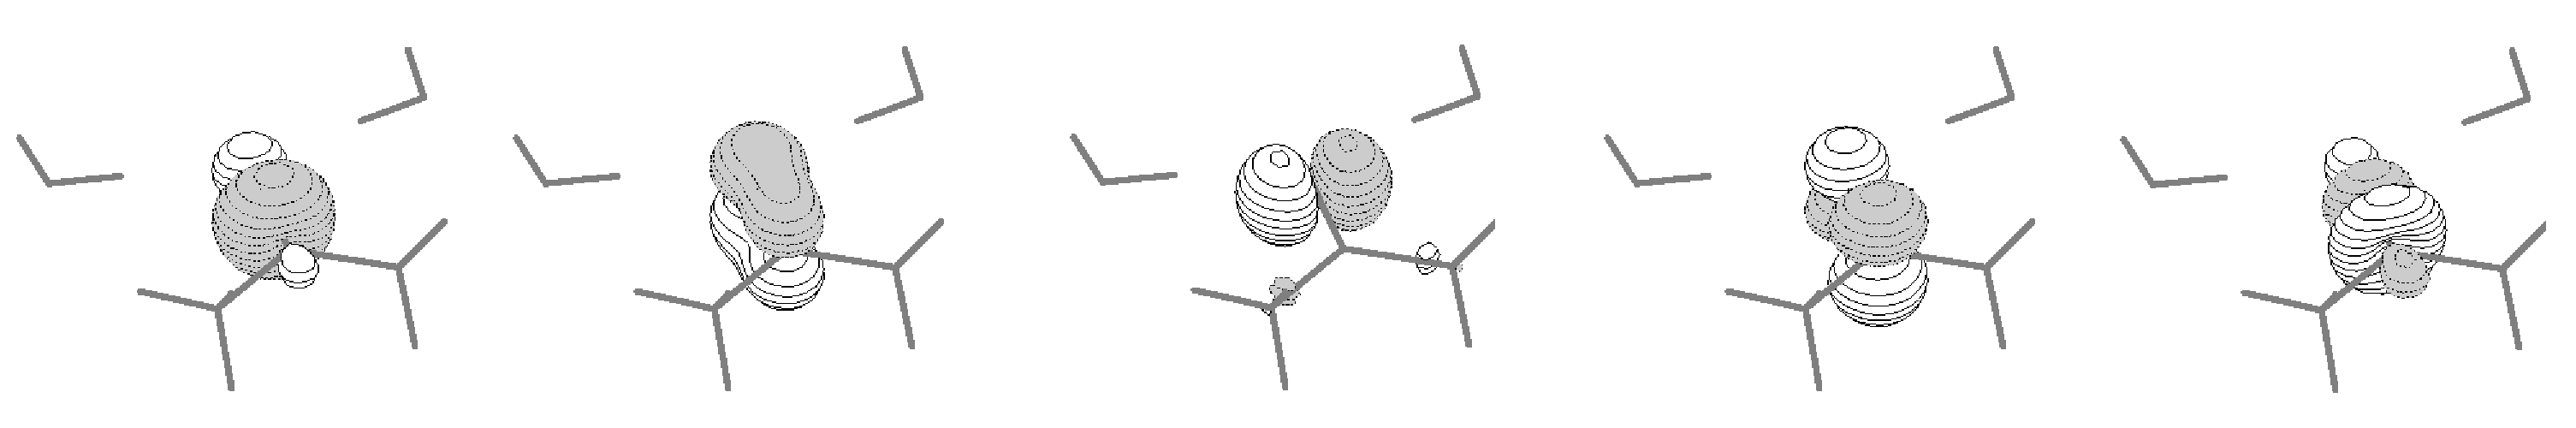
\includegraphics[width=11cm]{03_nevpt/images/h2o-active.eps}
\end{center}
\caption{\footnotesize The active orbitals for the evaluation on Acetone + 2
H$_2$O. From left to right, the $\sigma$, $\pi$, $n_y$, $\pi^{*}$,
$\sigma^{*}$. }
\label{fig:h2o-active}
\end{figure}
\end{center}


These orbitals are used in a Single-State NEVPT2 and a Non-Canonical
procedure, leading to the perturbative results presented in the left side
of Tab.~\ref{tbl:noncanonical}.  

\begin{center}
\begin{threeparttable}
\footnotesize
\begin{tabular*}{\textwidth}{l@{\hspace*{27mm}}cccc}
\hline
        & \multicolumn{2}{c}{Non-canonized} & \multicolumn{2}{c}{Canonized} \\
        &  SS-NEVPT     &  NC-NEVPT     &  SS-NEVPT     &  NC-NEVPT     \\
\hline
        &    \multicolumn{4}{c}{Ground State}\\
  (0)   & -0.1562219292 & -0.1610160883 & -0.1610160655 & -0.1610160655 \\
  (+1)  & -0.0060289124 & -0.0063728566 & -0.0063728572 & -0.0063728572 \\
  (-1)  & -0.0083210019 & -0.0084680922 & -0.0084680918 & -0.0084680918 \\
  (+2)  & -0.0021959738 & -0.0022262691 & -0.0022262691 & -0.0022262691 \\
  (-2)  & -0.0012134175 & -0.0011964952 & -0.0011964953 & -0.0011964954 \\
  (+1)' & -0.0011298902 & -0.0010747735 & -0.0010747734 & -0.0010747734 \\
  (-1)' & -0.0081324857 & -0.0080043857 & -0.0080043841 & -0.0080043842 \\
  (0)'  & -0.0095463813 & -0.0099518340 & -0.0099518346 & -0.0099518346 \\
\hline                                 
Total   & -0.1927899918 & -0.1983107946 & -0.1983107710 & -0.1983107711 \\
\hline                                 
        &    \multicolumn{4}{c}{\snpi}\\
\hline
  (0)   & -0.1569058671 & -0.1616113655 & -0.1616113419 &  -0.1616113419 \\
  (+1)  & -0.0089370064 & -0.0093753612 & -0.0093753625 &  -0.0093753624 \\
  (-1)  & -0.0059930216 & -0.0061061218 & -0.0061061209 &  -0.0061061209 \\
  (+2)  & -0.0009248766 & -0.0009503478 & -0.0009503479 &  -0.0009503479 \\
  (-2)  & -0.0002921853 & -0.0002913366 & -0.0002913366 &  -0.0002913366 \\
  (+1)' & -0.0043652467 & -0.0046995715 & -0.0046995705 &  -0.0046995704 \\
  (-1)' & -0.0025446880 & -0.0025151544 & -0.0025151554 &  -0.0025151554 \\
  (0)'  & -0.0117850231 & -0.0123542659 & -0.0123542653 &  -0.0123542652 \\
\hline
Total   & -0.1917479149 & -0.1979035247 & -0.1979035010 &  -0.1979035008 \\
\hline
\end{tabular*}
\caption{\footnotesize Comparison between the obtained contributions for the non-canonical technique.
The ``Non-canonized'' columns show the values obtained with non-canonical
localized orbitals using Partially Contracted Single-State NEVPT (SS-NEVPT)
and Non-Canonical NEVPT (NC-NEVPT).
The ``Canonized'' columns report the same evaluations, where a preliminar 
canonization of the localized orbitals has been performed. Both SS-NEVPT and
NC-NEVPT confirm the values obtained in the Non-canonized NC-NEVPT
evaluation.\label{tbl:noncanonical}
}
\end{threeparttable}
\end{center}

\vspace{4mm}

As can be seen, a non-negligible difference is present
between the obtained values.  Standard single-state NEVPT2 supposes the
non-diagonal elements of the Fock matrix as zero.  The \texttt{dypcNC}
program provides the highest non-diagonal element of the core and virtual
Fock matrixes

{
\footnotesize
\begin{verbatim}
 Maximum of off-diagonal core Fock matrix is   0.238695436106739
 Maximum of off-diagonal virtual Fock matrix is   8.252258688390988E-002
\end{verbatim}
}
which can be appreciated as non zero. This results in an error of the single
state treatment. 

The Non-Canonical evaluation keeps into account the non
diagonality of the Fock matrix, producing the correct value.
The correctness of this result is confirmed by canonizing the optimized
orbitals right before the perturbative evaluation. In this case, the
localization is lost, but the \texttt{dypcNC} confirms the diagonality of
the Fock matrix

{
\footnotesize
\begin{verbatim}
 Maximum of off-diagonal core Fock matrix is   6.924101073191773E-008
 Maximum of off-diagonal virtual Fock matrix is   4.398960914047209E-008
\end{verbatim}
}
and the obtained results (right side of Tab. \ref{tbl:noncanonical})
confirm the value obtained with the first evaluation.

A plot of the different nature of the orbitals used in the evaluation can be
seen in Fig. \ref{fig:h2o-orb}. The upper part of the figure shows an
extract of the localized set of non canonical orbitals, while the lower part plots
an extract of the orbitals after canonization. The delocalization of the
orbitals is clearly appreciable. 

\begin{center}
\begin{figure}[ht]
\begin{center}
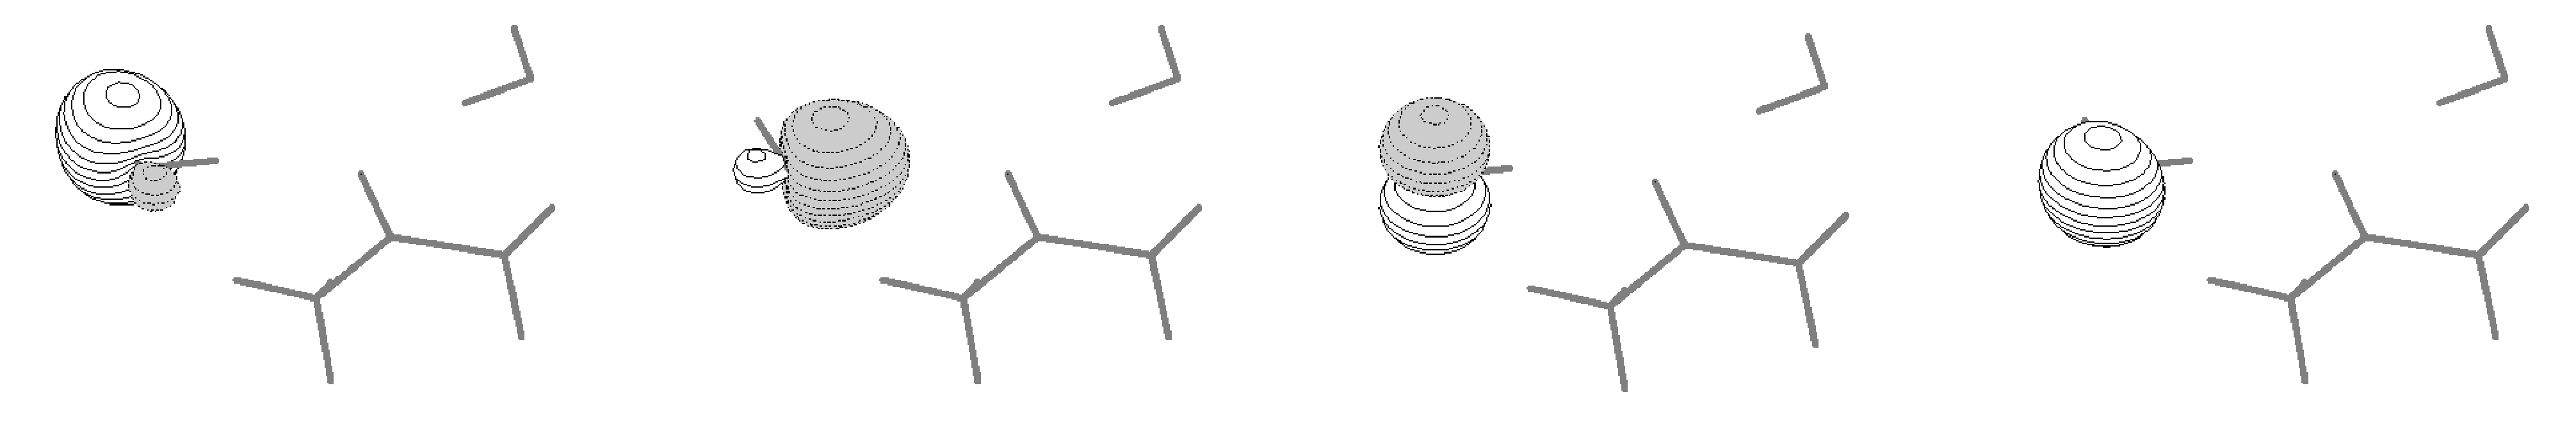
\includegraphics[width=11cm]{03_nevpt/images/h2o-loc.eps}
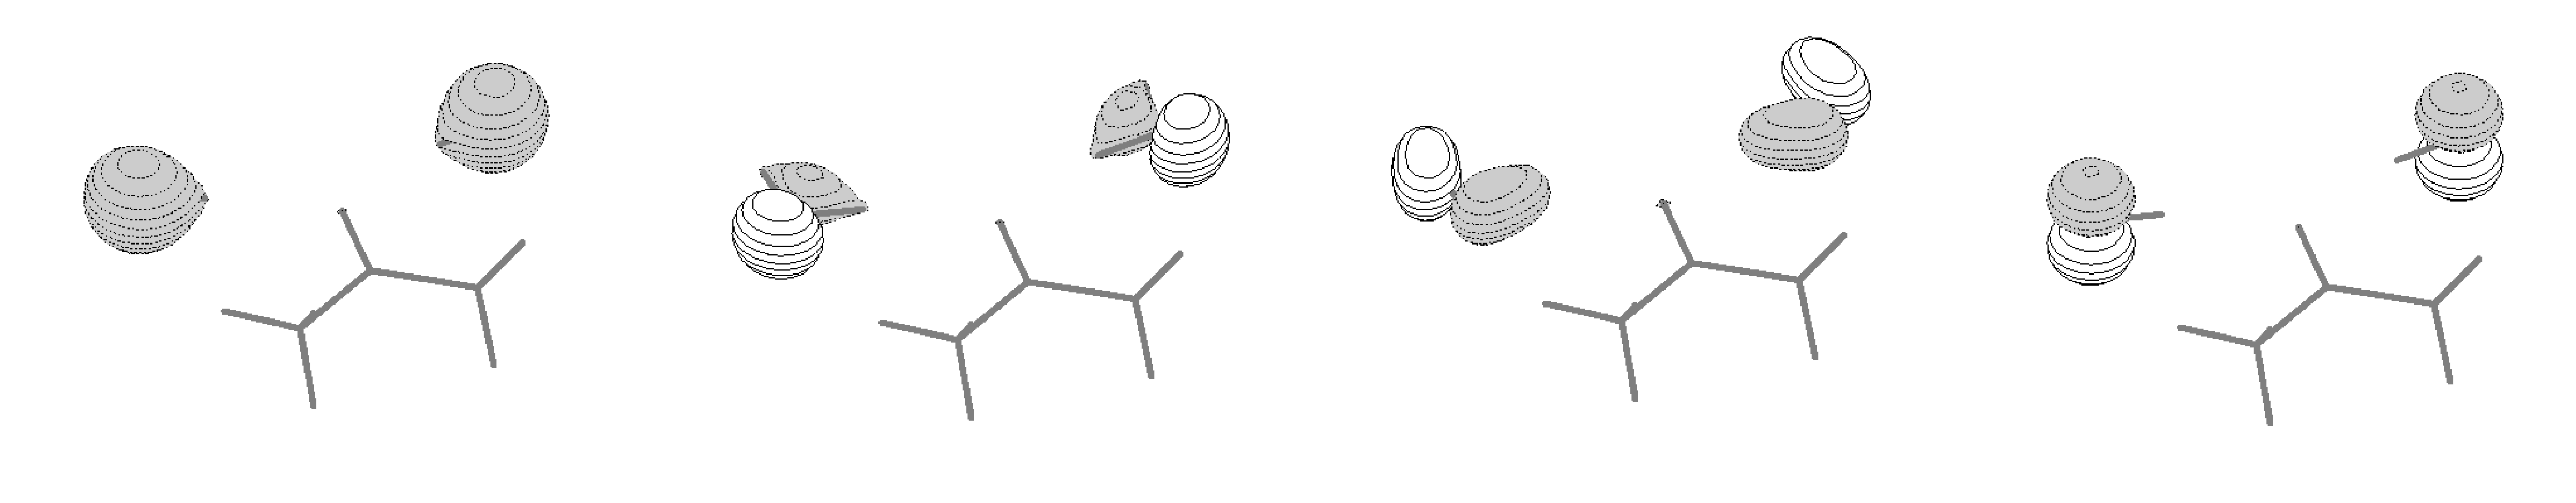
\includegraphics[width=11cm]{03_nevpt/images/h2o-deloc.eps}
\end{center}
\caption{\footnotesize A sample plot of non canonical localized orbitals
(upper part of the figure) and canonical delocalized orbitals (lower part)
for water orbitals. }
\label{fig:h2o-orb}
\end{figure}
\end{center}


Evaluating the energy difference provides consistency of the results.  For
the reported test, no high difference in the relative energies can be found,
as can be seen in Tab. \ref{tbl:noncanonical_energy}.

\begin{center}
\begin{threeparttable}
\begin{tabular*}{0.80\textwidth}{l@{\hspace*{27mm}}cccc}
\hline
        &  Ground   &  Excited    & Diff. \\
\hline
CASSCF   & -343.573883 & -343.411249 & 4.42 \\
SS-NEVPT & -343.766673 & -343.602997 & 4.45 \\
NC-NEVPT & -343.772194 & -343.609153 & 4.43 \\
\hline                                 
\end{tabular*}
\caption{\footnotesize Absolute energies and their differences for the
acetone+2 H$_2$O system. From the comparison of the relative excitation
energies, no high differencies between the methods can be found in the
analyzed system.
}
\label{tbl:noncanonical_energy}
\end{threeparttable}
\end{center}


This must be further investigated, given the small basis set used. However,
the target of this investigation was to demonstrate the consistency of the
NC-NEVPT results.

